A brief introduction to this chapter.

\section{Motivation}

Sample citations: pre-trained GPT-2\footnote{Codes available at \url{https://github.com/lileipisces/PEPLER}} \cite{22-PEPLER}, Transformer \cite{ACL21-PETER}, \gls*{rnn} \cite{CIKM20-NETE}

\section{Outline}

\section{Contributions}

\begin{figure}
	\centering
	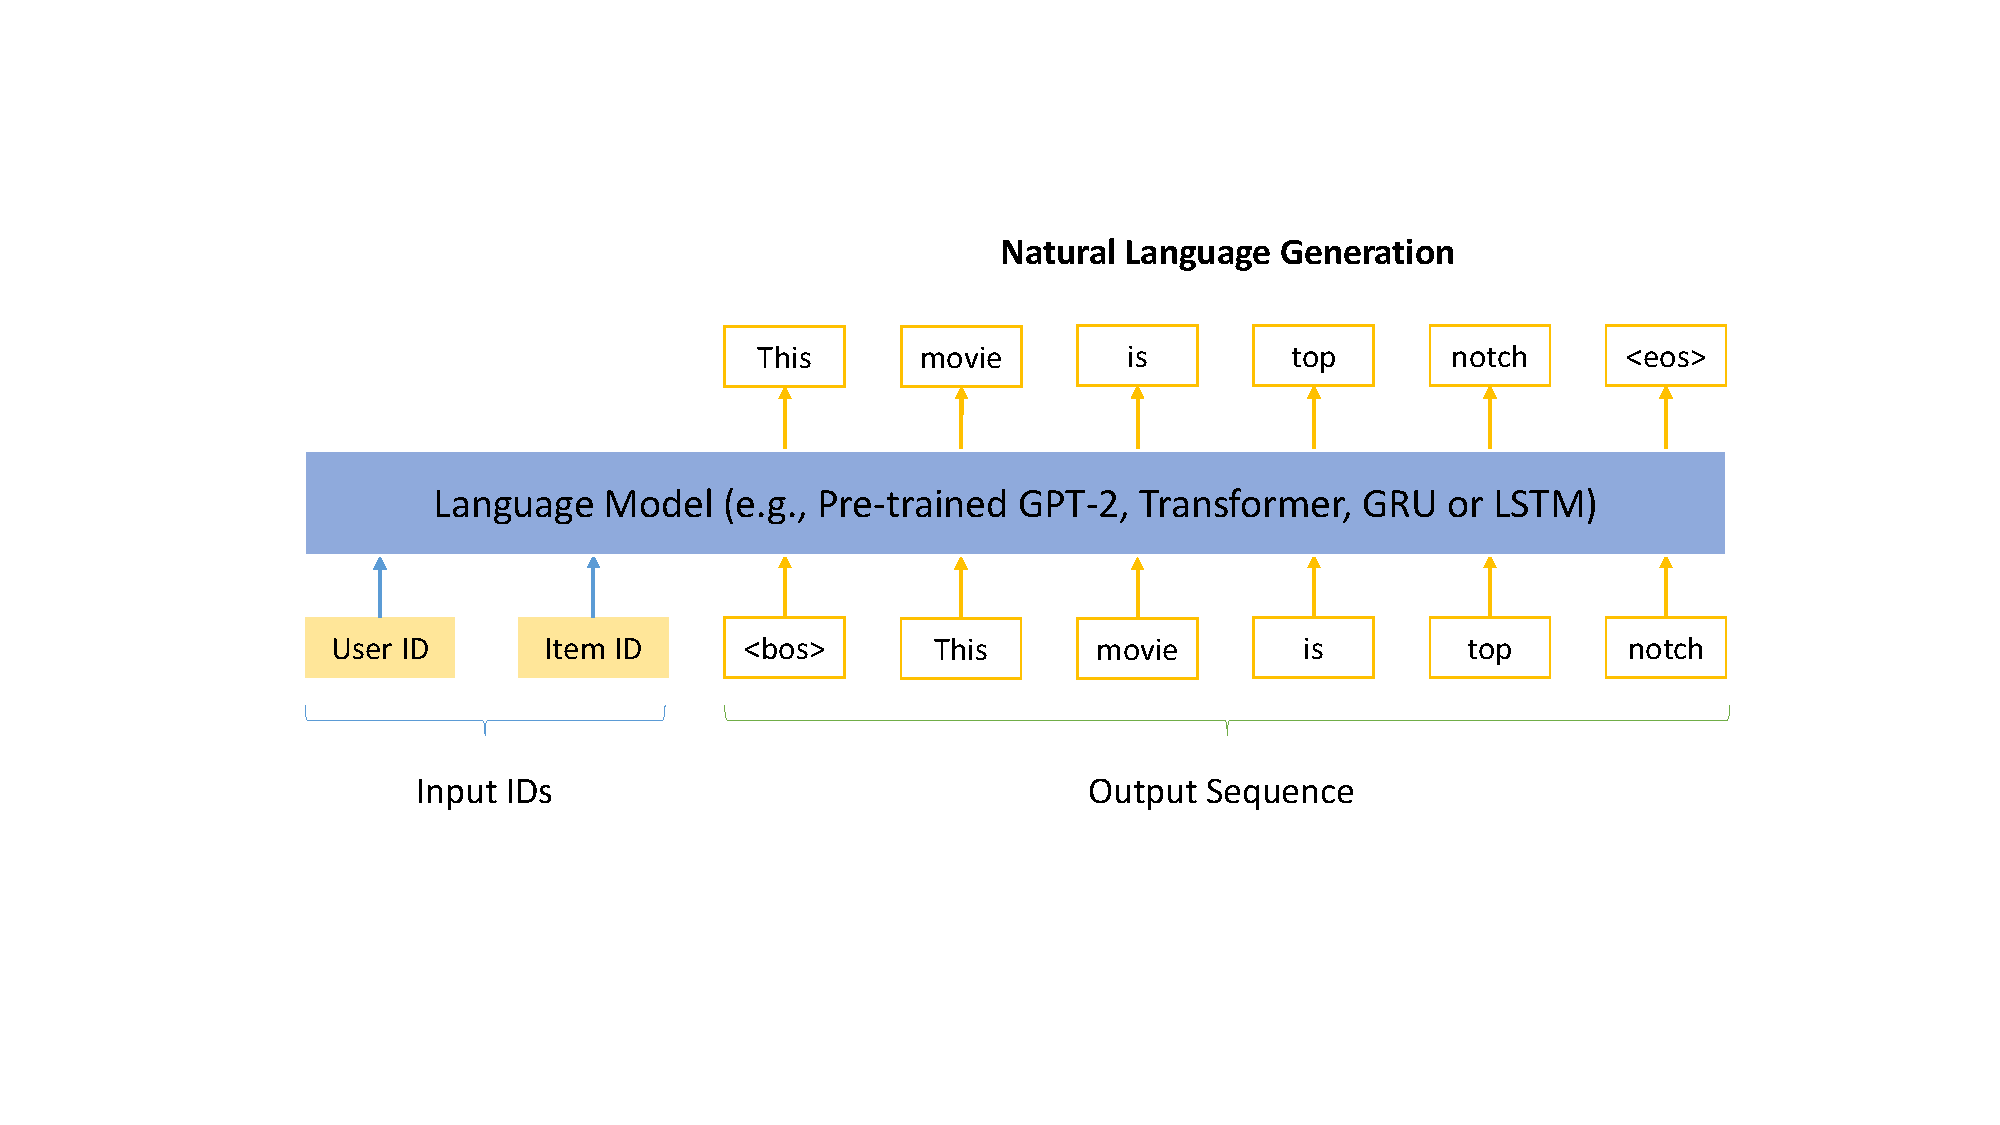
\includegraphics[scale=0.5]{fig/ch1/NLG4RS.pdf}
	\caption[Overview of recommender systems-based natural language generation.]{Overview of recommender systems-based natural language generation. In the case of recommendation explanation generation, the model is instructed to generate a word sequence for explaining why an item is recommended to the user.}
	\label{fig1:model}
\end{figure}

Use the following command to shorten the captions shown in List of Tables/Figures:
\begin{verbatim}
	\caption[shorter caption in List of
	Tables/Figures]{Real capation above or below the table/figure}
\end{verbatim}
See Fig. \ref{fig1:model} for example.
